\section{Interface}
\label{sec:mockups}

Nesta seção será apresentadas as telas do sistema, tanto para digitalização de novos documentos quanto para a configuração de {\it scanners}. Na seção \ref{sec:mockups_digitalizar}, tem-se os passos para digitalizar um novo documento (storyboard) e as telas que o sistema apresentará para o usuário (mockups). Na seção seguinte (seção \ref{sec:mockups_configurar}), tem-se as telas para configuração de {\it scanners}.

%%%%%%%%%%%%%%%%%%%%%%%%%%%%%%%%%%%%%%%%%%%%%%%%%%%%%%%%%%%%%%%%%%%
\subsection{Digitalizar Documento}
\label{sec:mockups_digitalizar}

Ao iniciar o sistema, o usuário é apresentado com a tela na figura \ref{fig:dig_1}. É interessante destacar o aviso no topo da tela, mostrando que o sistema está procurando por {\it scanners} instalados e configurados no sistema.

\begin{figure}[h]
 \centering
    \setlength\fboxsep{0pt}
    \setlength\fboxrule{0.5pt}
    \fbox{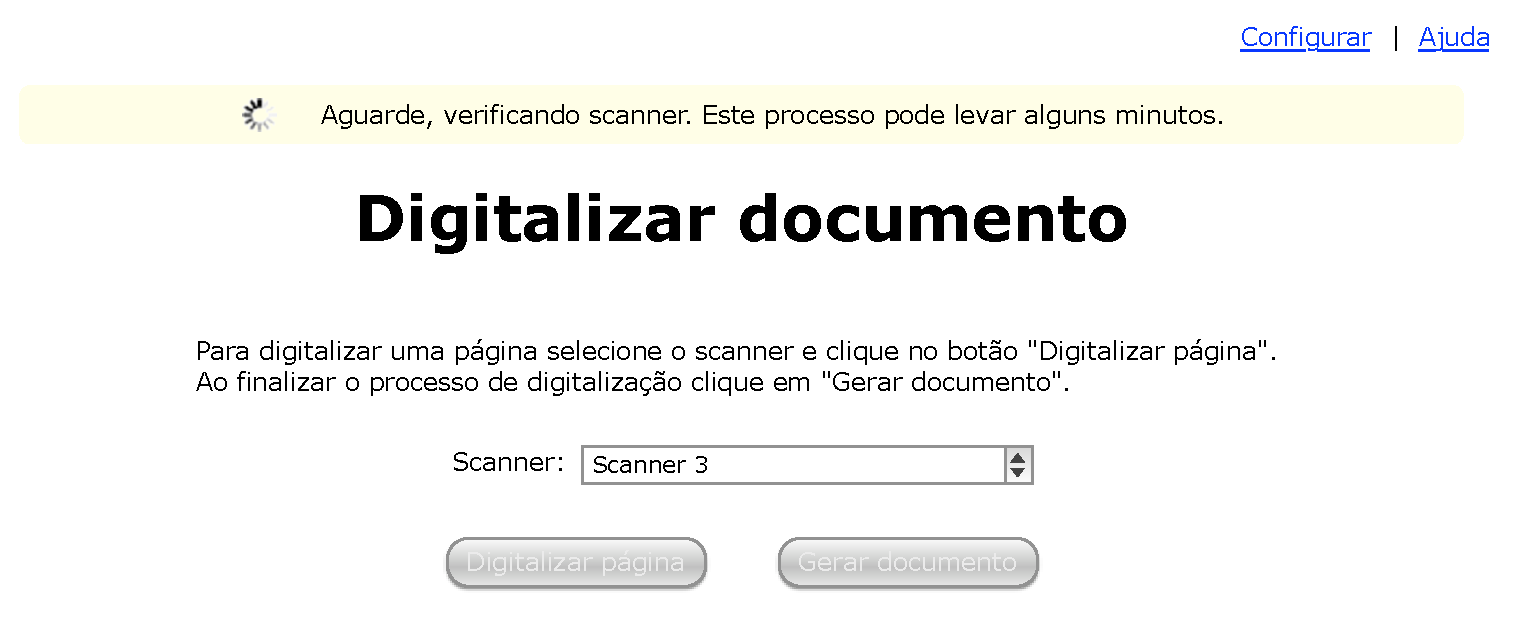
\includegraphics[scale=0.6]{img/mockups/digitalizacao-1.pdf}}
  \caption {Tela inicial do sistema}
  \label{fig:dig_1}
\end{figure}

Caso não haja nenhum {\it scanner} configurado no sistema, um aviso é apresentado ao usuário, pedindo a ele configure o {\it scanner} selecionado para ser usado pelo sistema.

\begin{figure}[h]
 \centering
    \setlength\fboxsep{0pt}
    \setlength\fboxrule{0.5pt}
    \fbox{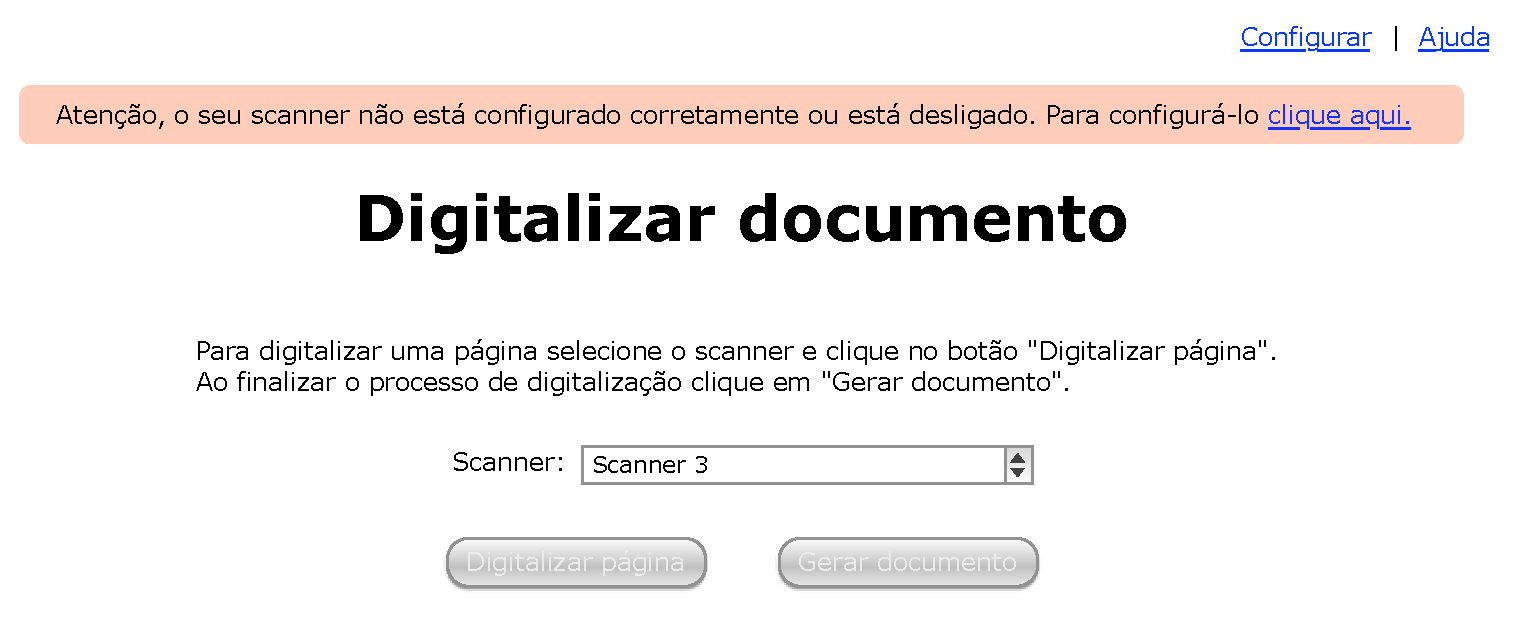
\includegraphics[scale=0.6]{img/mockups/digitalizacao-2.pdf}}
  \caption {Tela indiciando erro: o {\it scanner} selecionado não está corretamente configurado ou não está ligado}
  \label{fig:dig_2}
\end{figure}

Se o {\it scanner} estiver corretamente configurado e ligado, o usuário pode iniciar a criação de um novo documento, clicando no botão ``Digitalizar página'', apresentado na figura \ref{fig:dig_3}. Nessa situação, o botão ``Gerar documento'' está desativado e emite uma mensagem caso o usuário tente clicá-lo.

\begin{figure}[h]
 \centering
    \setlength\fboxsep{0pt}
    \setlength\fboxrule{0.5pt}
    \fbox{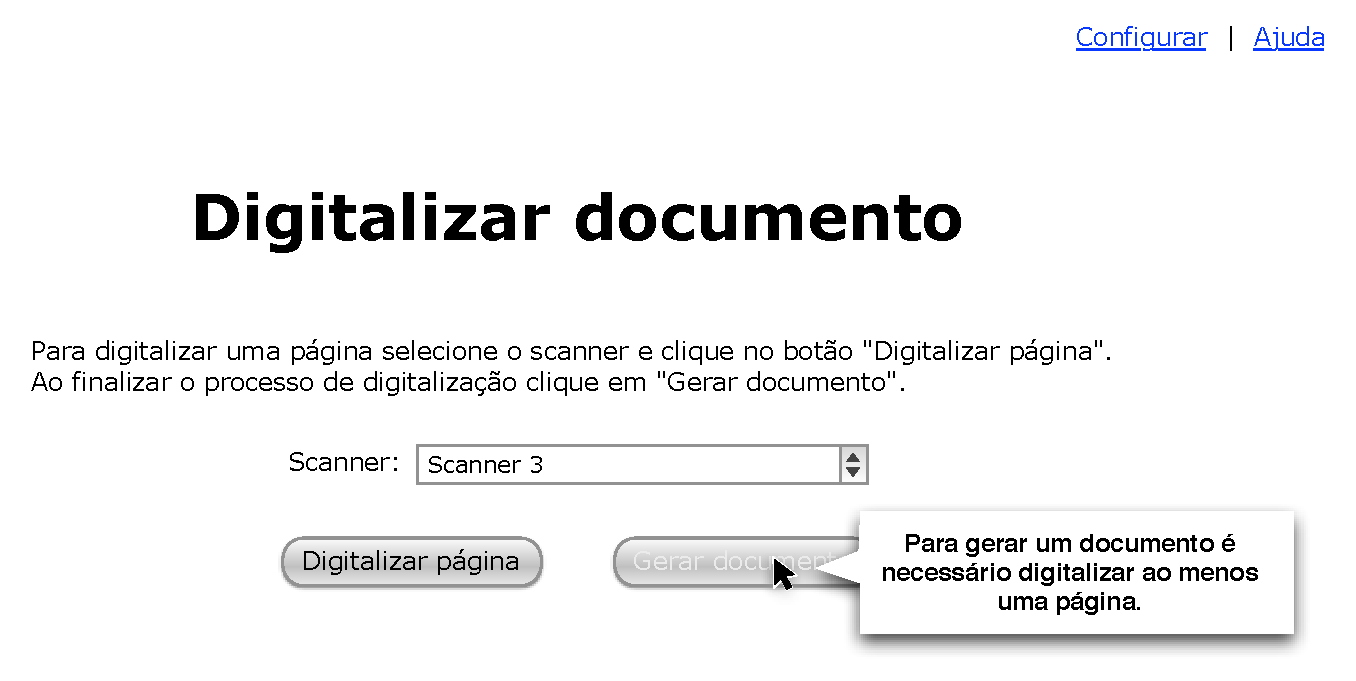
\includegraphics[scale=0.6]{img/mockups/digitalizacao-3.pdf}}
  \caption {Tela indicando o sistema está pronto e o usuário pode começar a digitalizar documentos}
  \label{fig:dig_3}
\end{figure}

Após clicar no botão ``Digitalizar página'', o é apresentada para o usuário uma mensagem para que ele espere a digitalização do documento que está no {\it scanner}, na tela apresentada na figura \ref{fig:dig_4}.

\begin{figure}[h]
 \centering
    \setlength\fboxsep{0pt}
    \setlength\fboxrule{0.5pt}
    \fbox{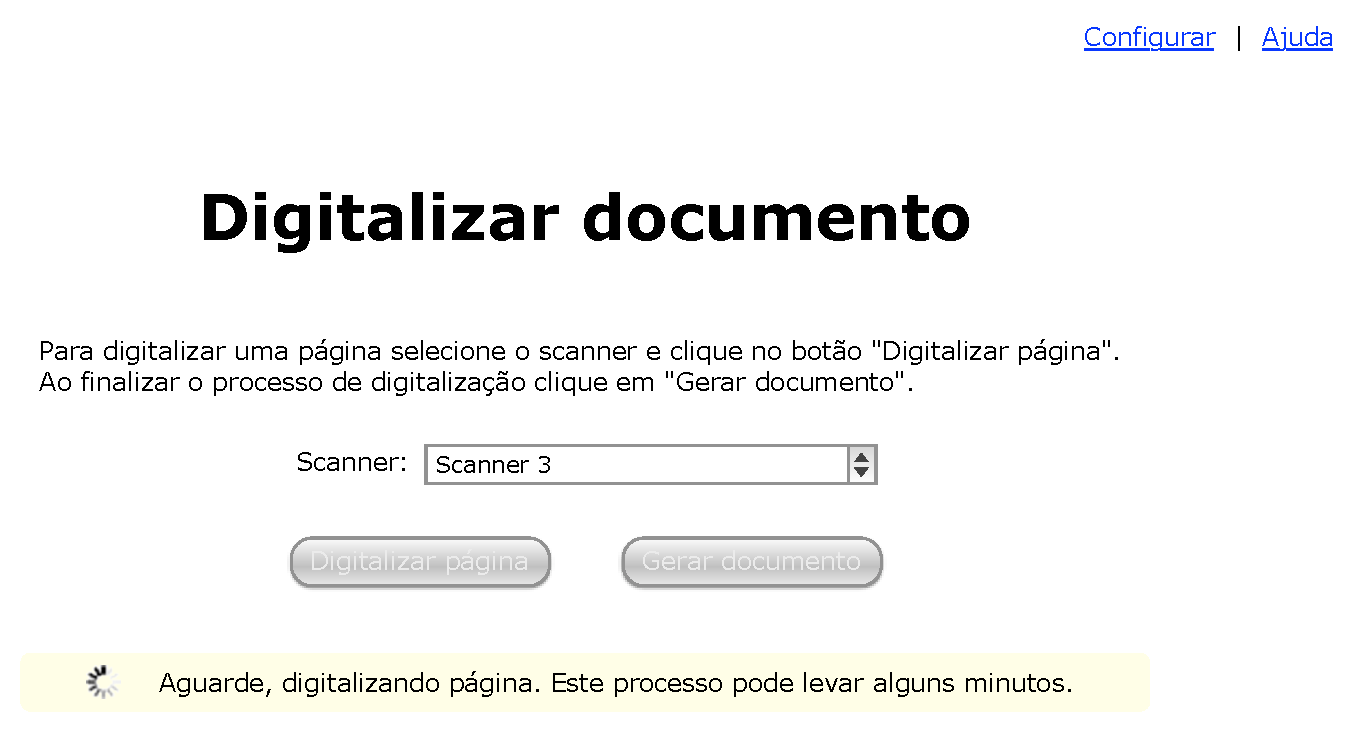
\includegraphics[scale=0.6]{img/mockups/digitalizacao-4.pdf}}
  \caption {Tela indicando que uma página está sendo digitalizada}
  \label{fig:dig_4}
\end{figure}

Em seguida, na figura \ref{fig:dig_5}, após a digitalização de várias páginas, é exibida pequenas amostras das páginas já digitalizadas e um marcador, indicando se a página deverá ser incluída no novo documento ou não. Após a seleção das páginas, o usuário deve clicar no botão ``Gerar documento''.

\begin{figure}[h]
 \centering
    \setlength\fboxsep{0pt}
    \setlength\fboxrule{0.5pt}
    \fbox{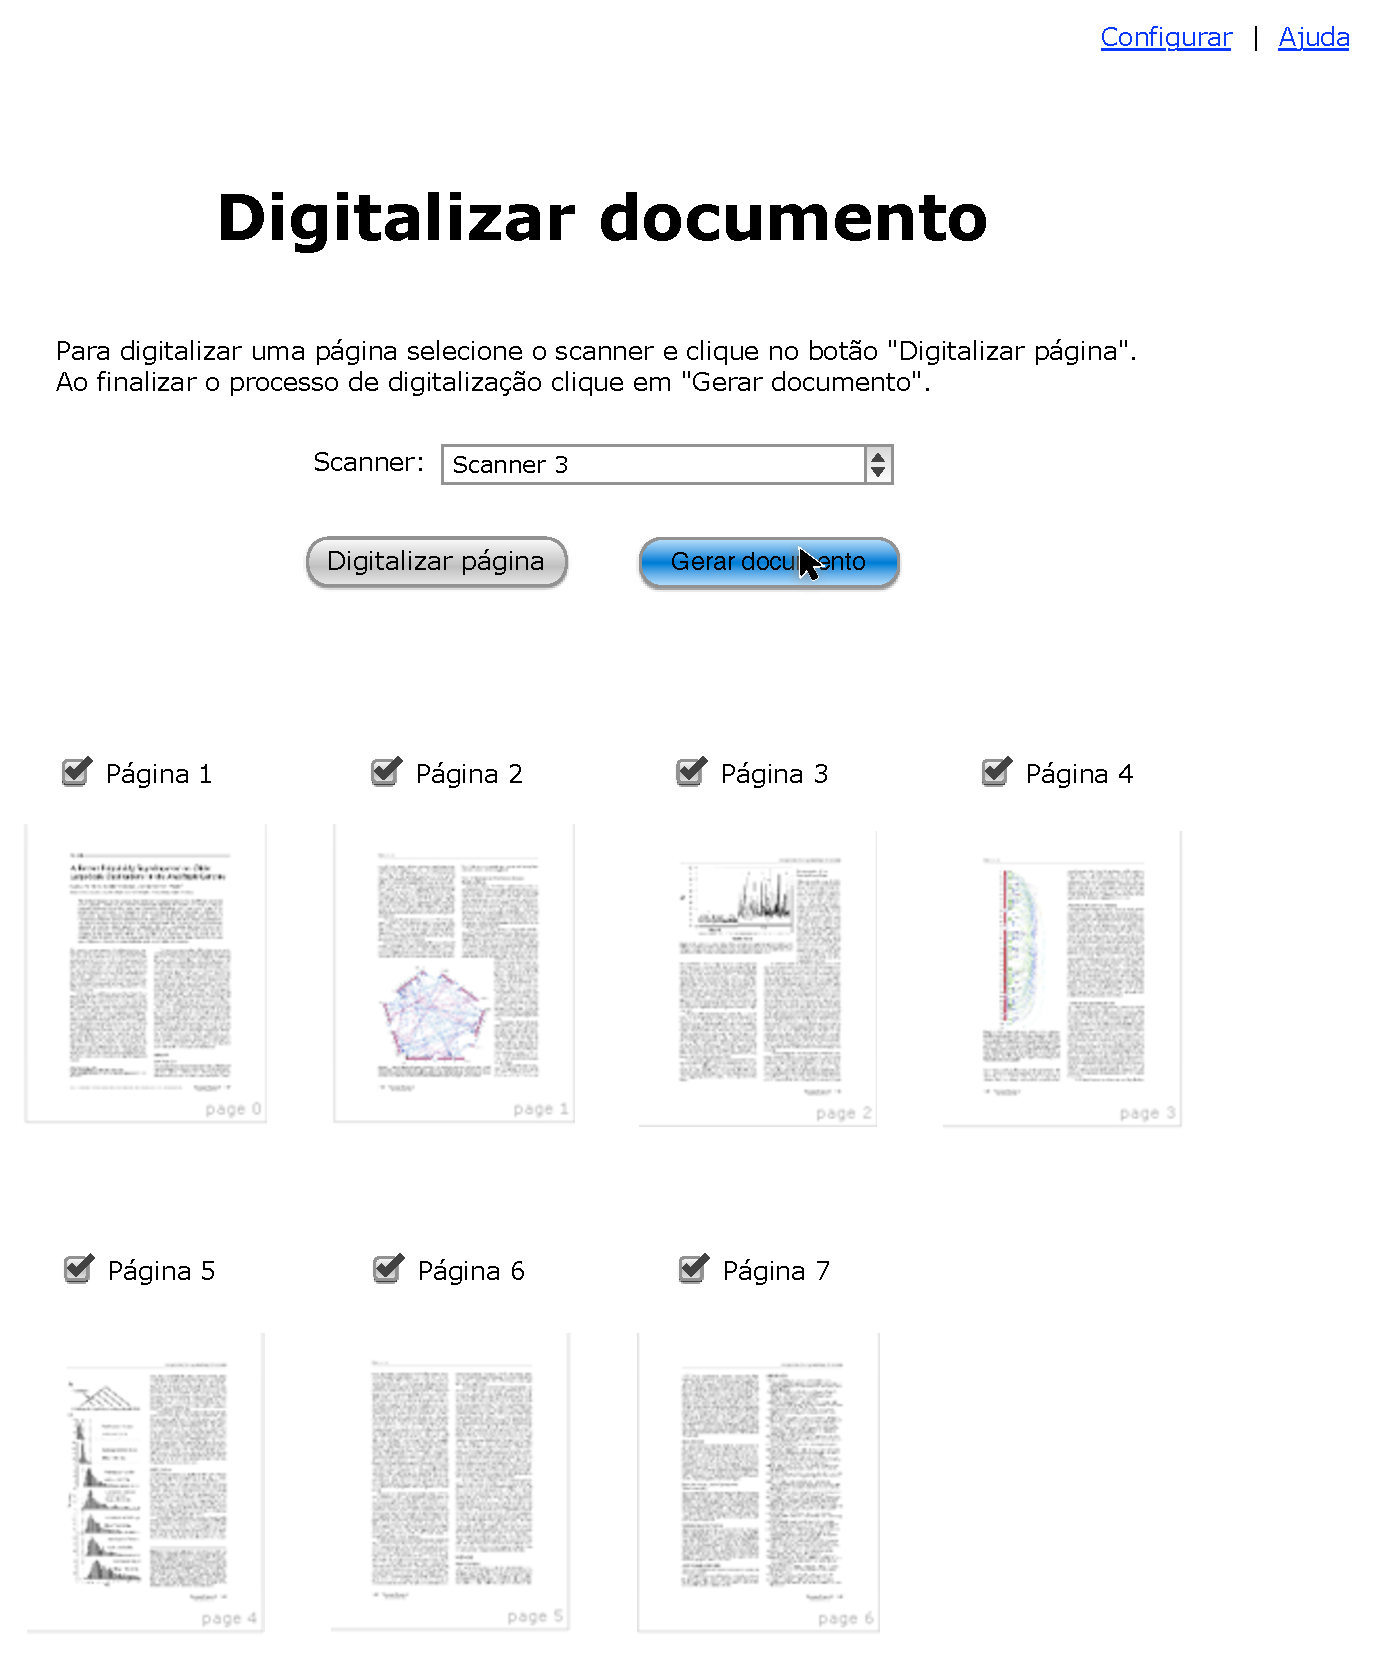
\includegraphics[scale=0.6]{img/mockups/digitalizacao-5.pdf}}
  \caption {Tela mostrando amostras das páginas já digitalizadas}
  \label{fig:dig_5}
\end{figure}

No próximo passo, representado pela figura \ref{fig:dig_6}, o usuário deve escolher então um nome para o documento e uma breve descrição sobre ele. A descrição deste novo documento é opcional.

\begin{figure}[h]
 \centering
    \setlength\fboxsep{0pt}
    \setlength\fboxrule{0.5pt}
    \fbox{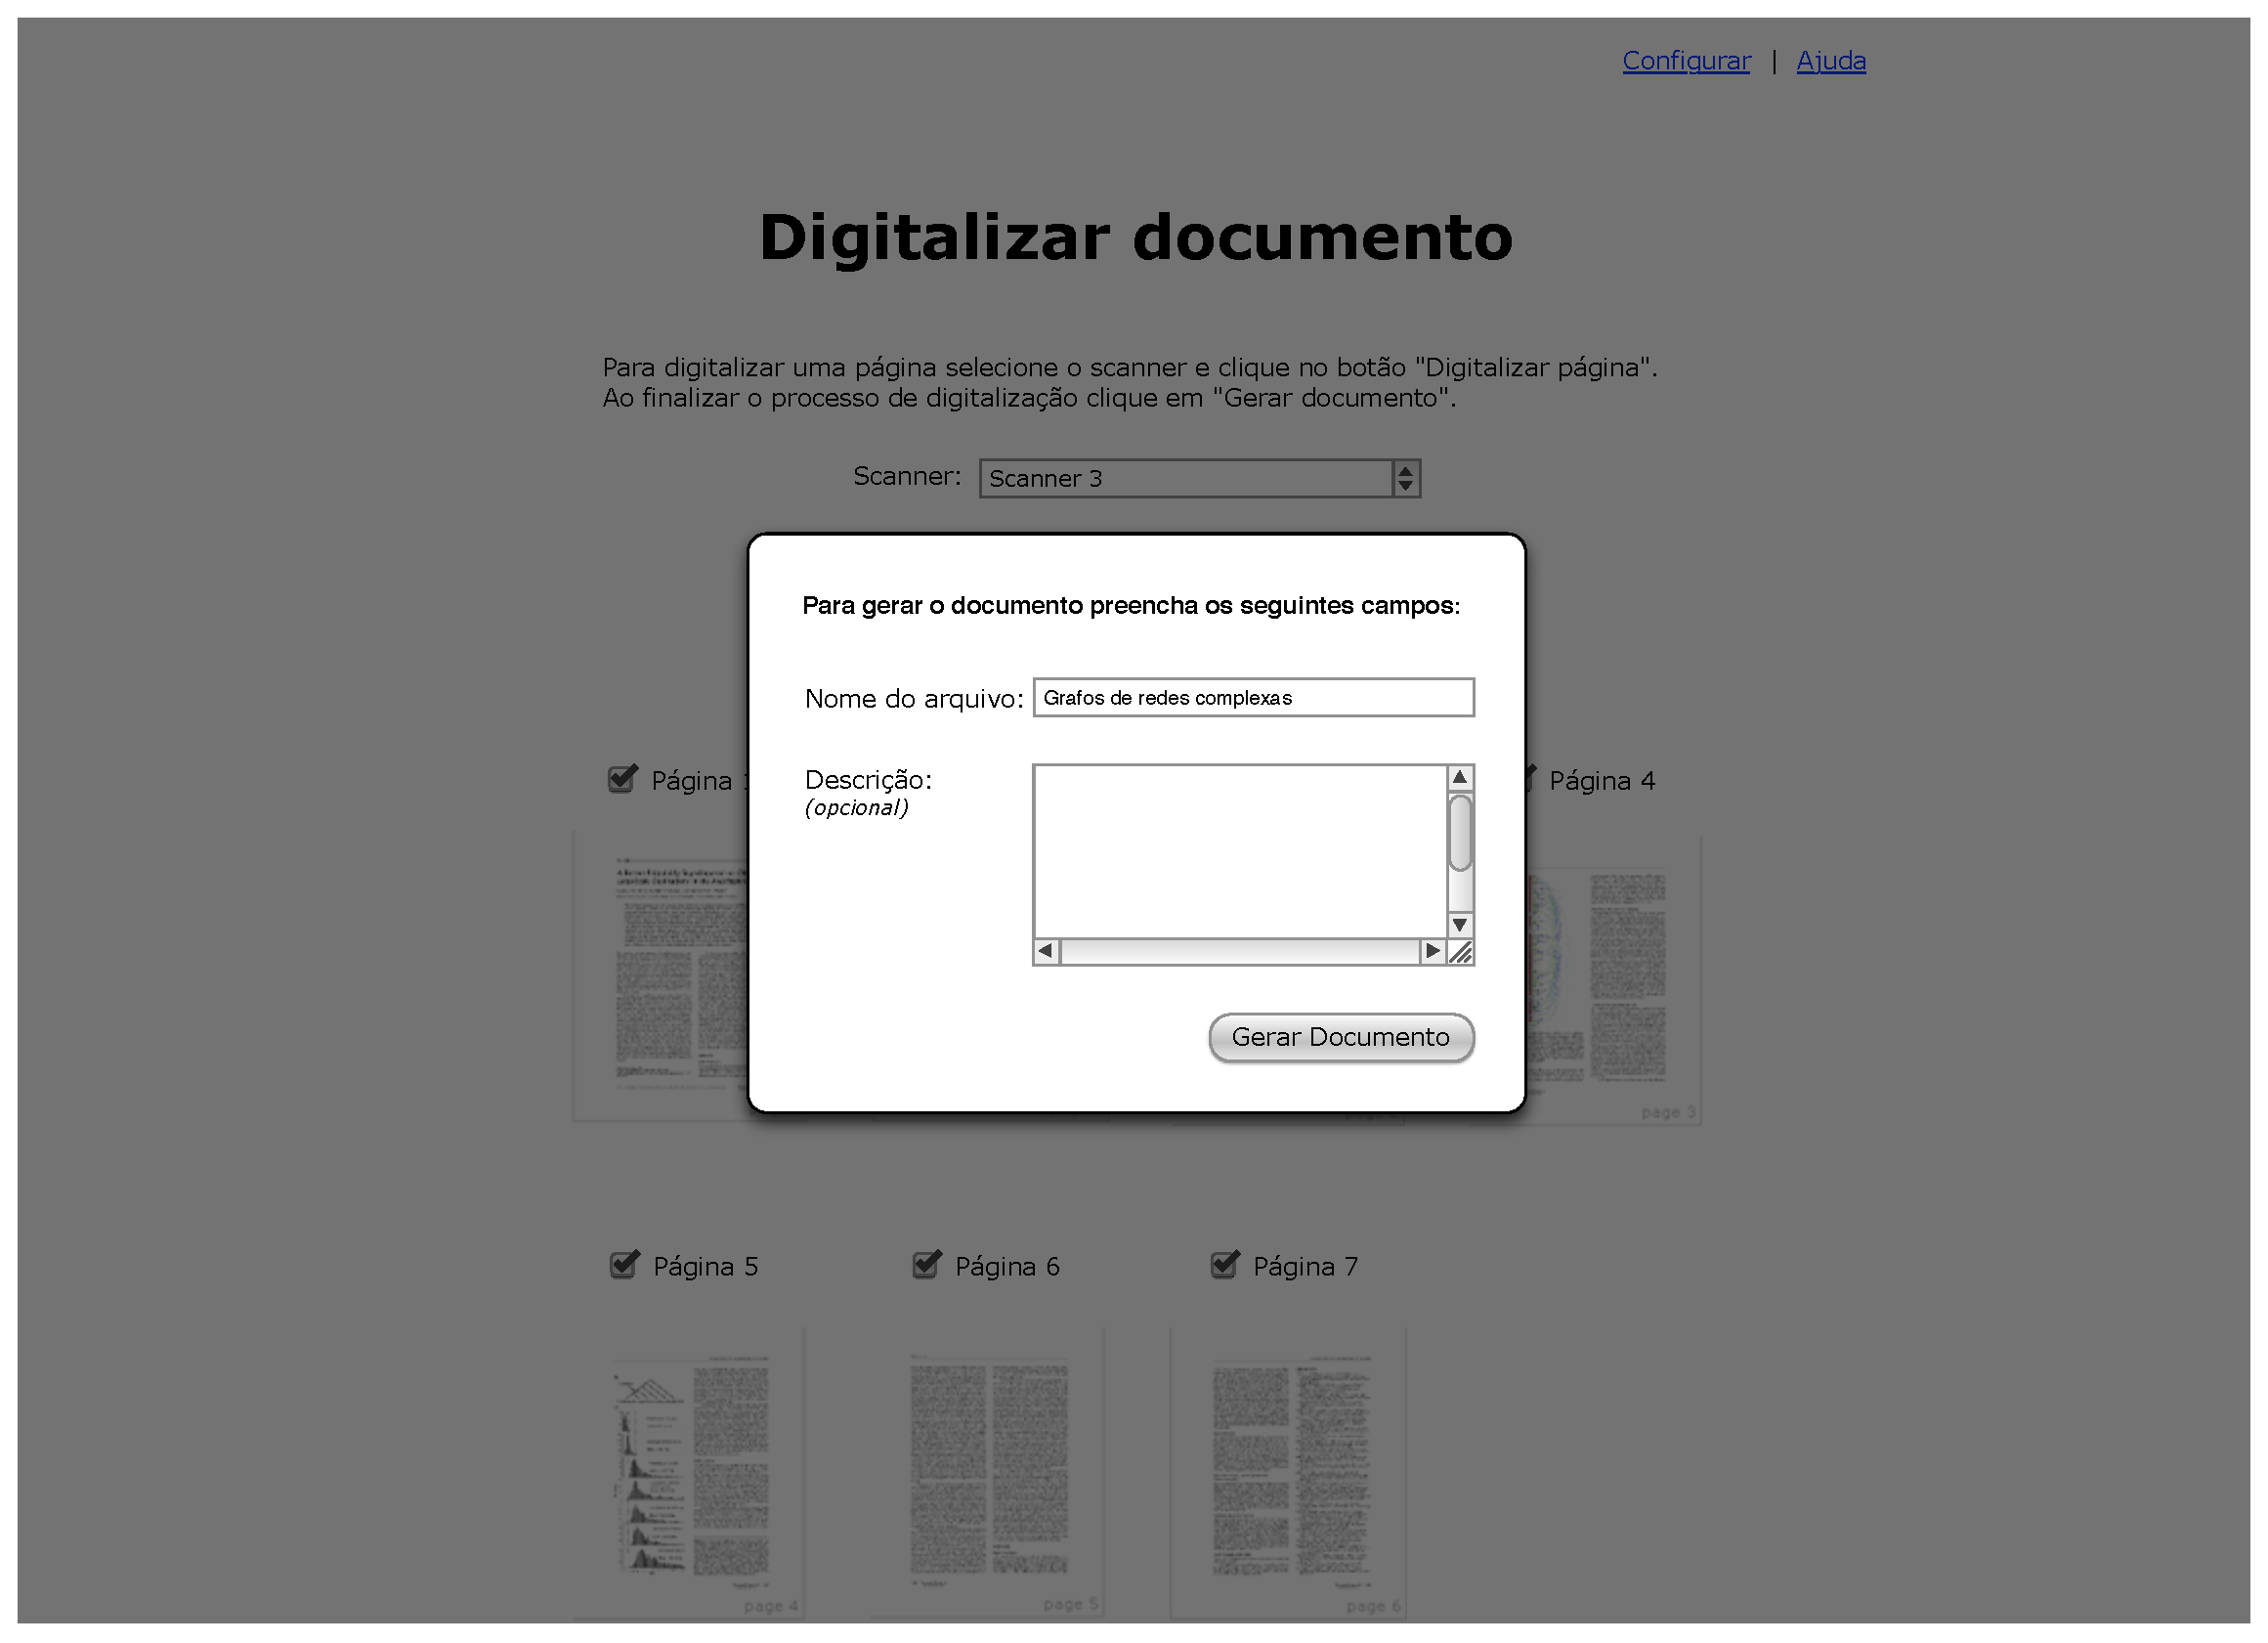
\includegraphics[scale=0.4]{img/mockups/digitalizacao-6.pdf}}
  \caption {Tela para a entrada de um nome e descrição para o novo documento}
  \label{fig:dig_6}
\end{figure}

Finalmente, após a criação do documento, o sistema mostra uma confirmação da criação do documento (figura \ref{fig:dig_7}) e indica seu estado. No exemplo, o sistema está pronto para digitalizar um novo documento.

\begin{figure}[h]
 \centering
    \setlength\fboxsep{0pt}
    \setlength\fboxrule{0.5pt}
    \fbox{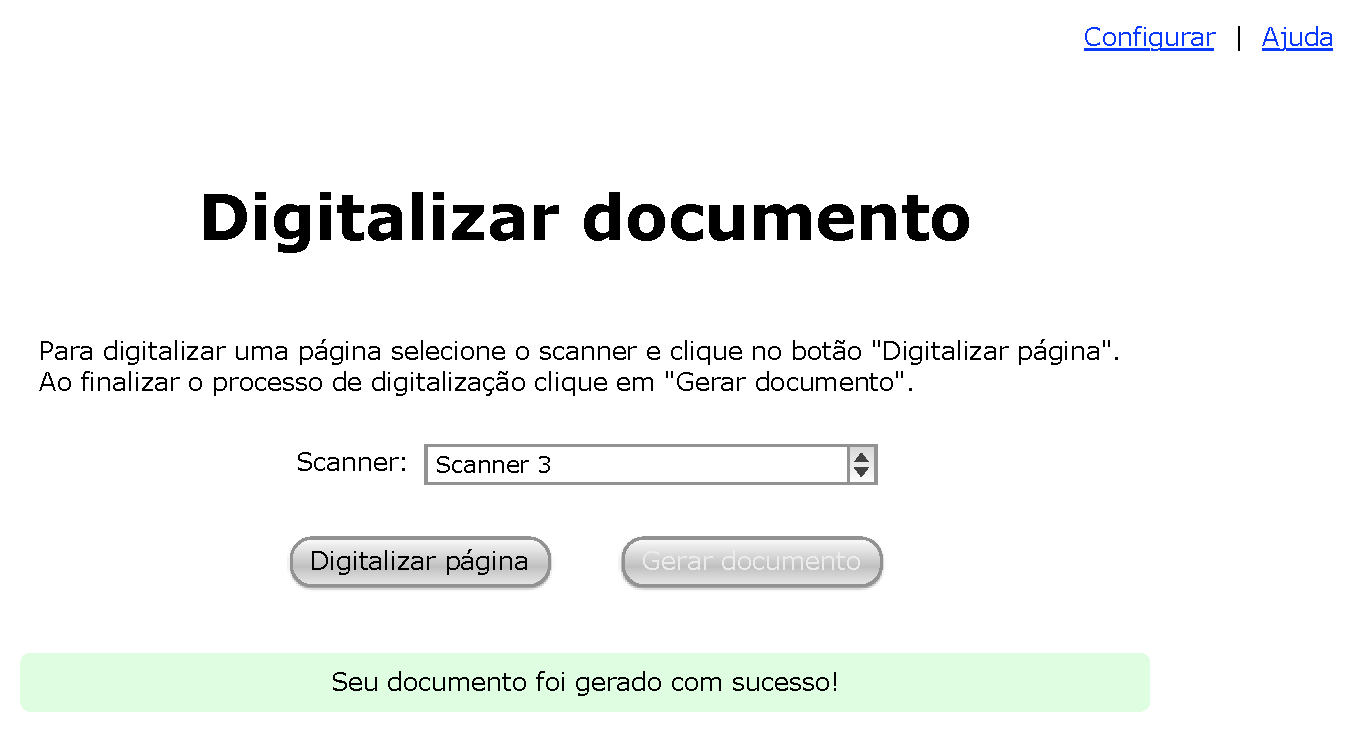
\includegraphics[scale=0.6]{img/mockups/digitalizacao-7.pdf}}
  \caption {Tela confirmando a criação de um novo documento}
  \label{fig:dig_7}
\end{figure}

A figura \ref{fig:dig_8} mostra a tela no caso em que o usuário digitalizou páginas anteriormente, porém não gerou um documento. Essas páginas ficam armazenadas no sistema e, logo que ele tente digitalizar novos documentos, poderá decidir se quer usar as páginas previamente digitalizadas ou descartá-las, para gerar um novo documento.

\begin{figure}[h]
 \centering
    \setlength\fboxsep{0pt}
    \setlength\fboxrule{0.5pt}
    \fbox{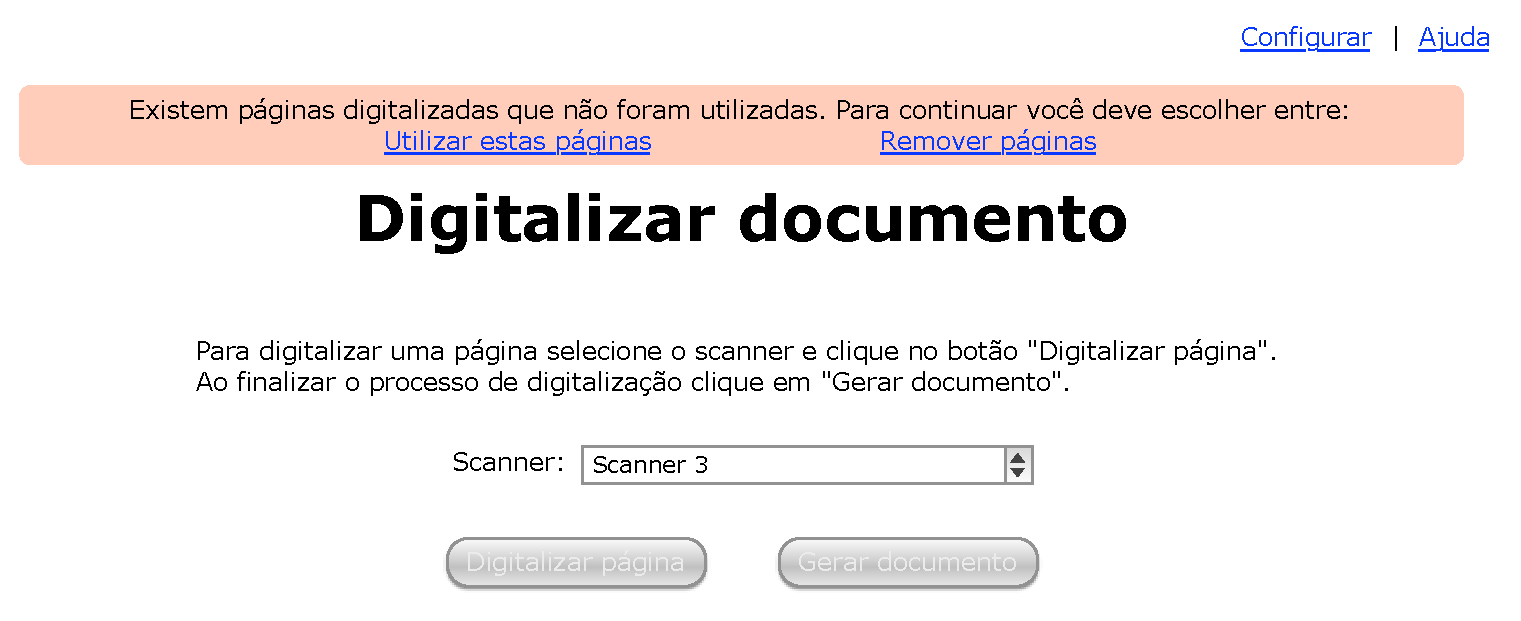
\includegraphics[scale=0.6]{img/mockups/digitalizacao-8.pdf}}
  \caption {Tela mostrando a situação de páginas previamente digitalizadas}
  \label{fig:dig_8}
\end{figure}



%%%%%%%%%%%%%%%%%%%%%%%%%%%%%%%%%%%%%%%%%%%%%%%%%%%%%%%%%%%%%%%%%%%%
\subsection{Configurar Scanner}
\label{sec:mockups_configurar}

Ao clicar no {\it link} ``Configurações'', o ususário deve selecionar qual {\it scanner} ele deseja configurar. Na tela \ref{fig:config_1}, é possível ver uma tela que mostra a escolha de um dispositivo para configuração.

\begin{figure}[h]
 \centering
    \setlength\fboxsep{0pt}
    \setlength\fboxrule{0.5pt}
    \fbox{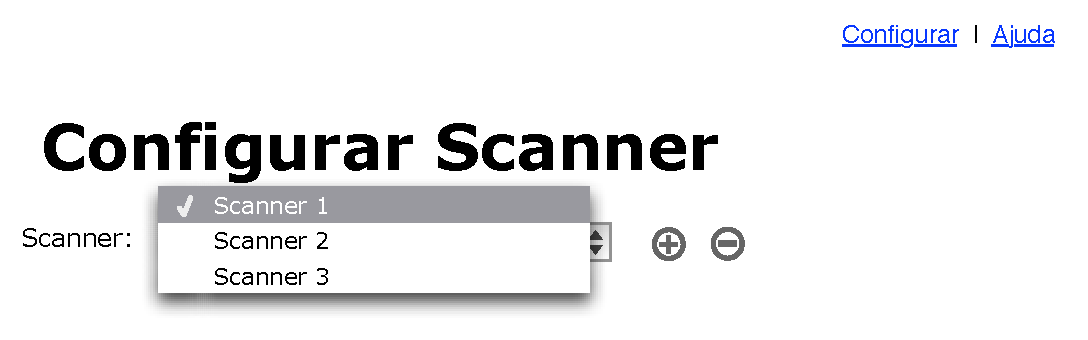
\includegraphics[scale=0.6]{img/mockups/config-1.pdf}}
  \caption {Tela mostrando a seleção de {\it scanners} para configuração}
  \label{fig:config_1}
\end{figure}

Após a escolha do {\it scanner}, o usuário encontra a tela exibida na figura \ref{fig:config_2}, na qual encontram-se campos para configuração do dispositivo, como tamanho da página, nome e modelo do {\it scanner}. É interessante notar os botões ``+'' e ``-'', para a adição e remoção de {\it scanners}, respectivamente.

\begin{figure}[h]
 \centering
    \setlength\fboxsep{0pt}
    \setlength\fboxrule{0.5pt}
    \fbox{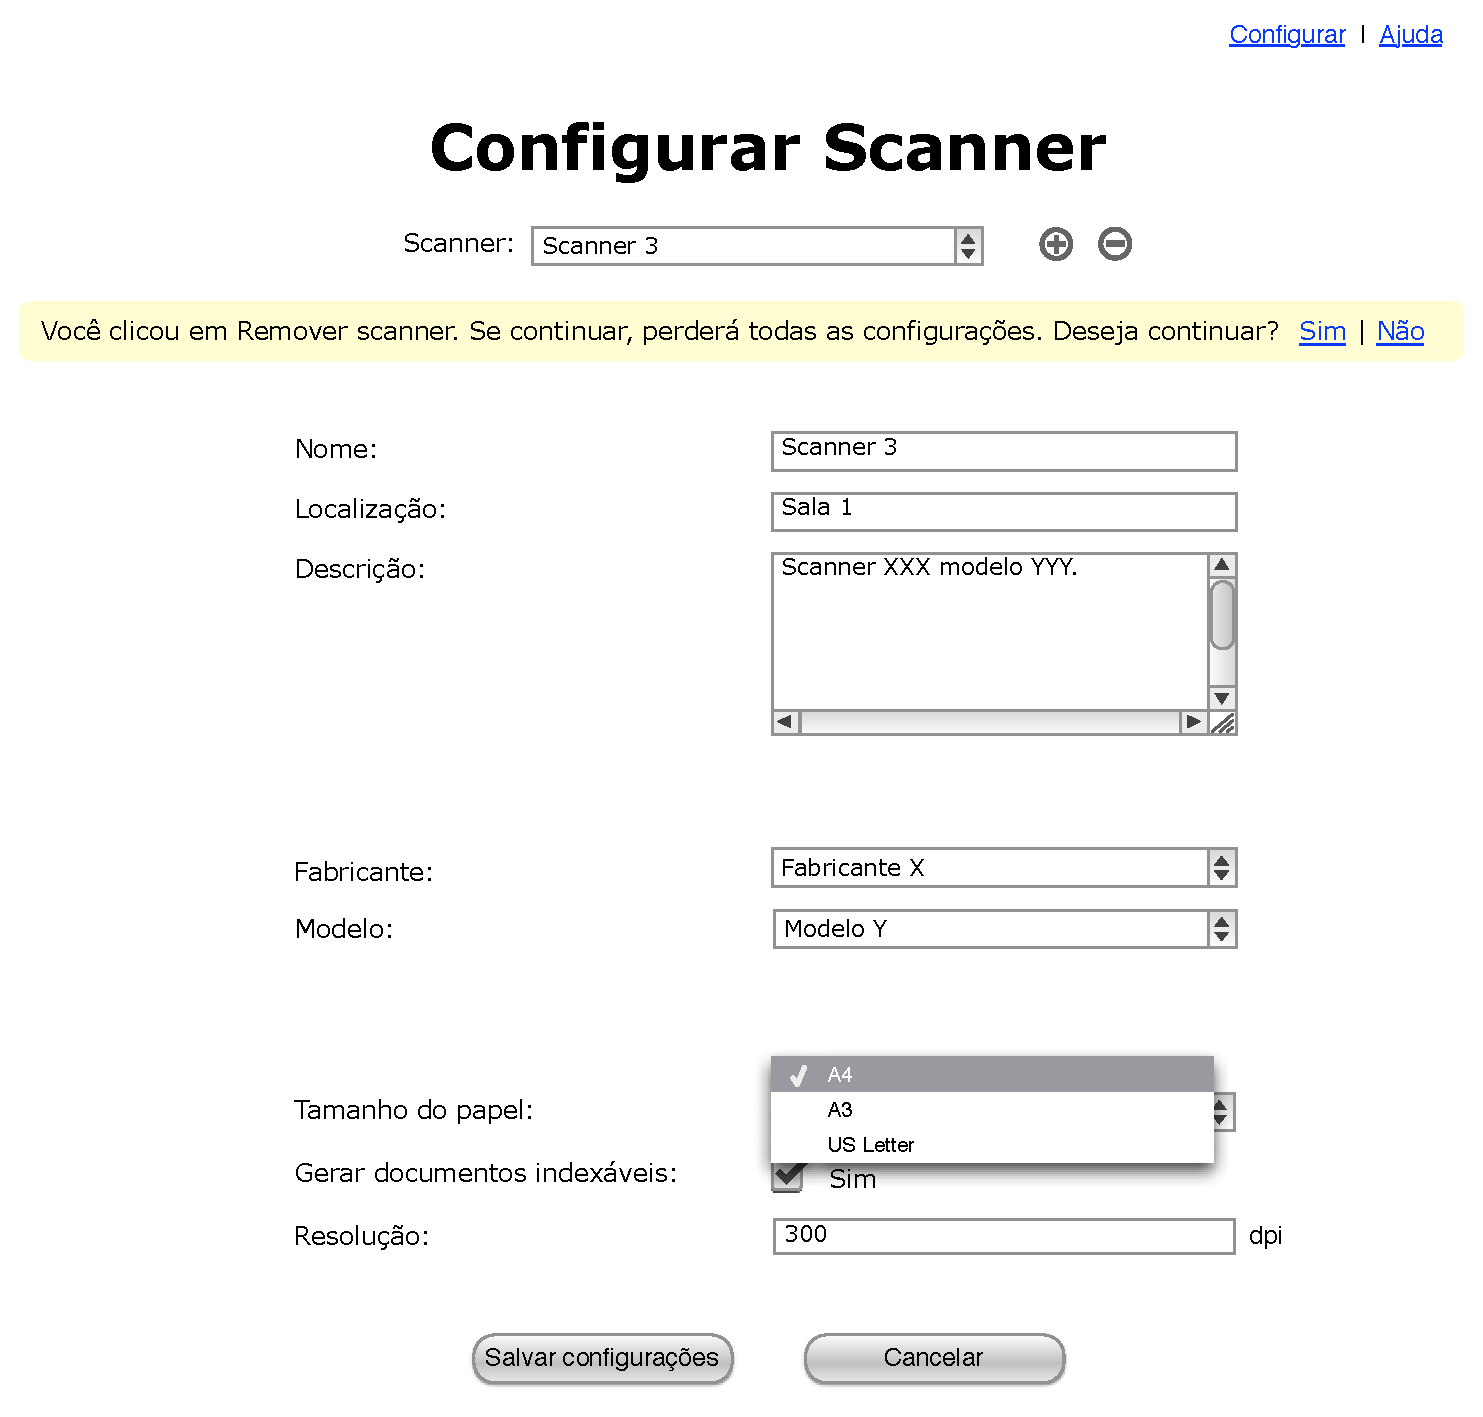
\includegraphics[scale=0.6]{img/mockups/config-2.pdf}}
  \caption {Tela mostrando as configurações de um {\it scanner}}
  \label{fig:config_2}
\end{figure}
